% Template for ICIP-2017 paper; to be used with:
%          spconf.sty  - ICASSP/ICIP LaTeX style file, and
%          IEEEbib.bst - IEEE bibliography style file.
% --------------------------------------------------------------------------
\documentclass{article}
\usepackage{spconf,amsmath,graphicx}
\usepackage{pbox}
\usepackage{subcaption}
\usepackage{float}
\usepackage{cite}

% Example definitions.
% --------------------
\def\x{{\mathbf x}}
\def\L{{\cal L}}

% Title.
% ------
\title{AUTHOR GUIDELINES FOR ICIP 2017 PROCEEDINGS MANUSCRIPTS}
%
% Single address.
% ---------------
% \name{No\'{e} Le Philippe, Vincent Itier, William Puech}
% \address{Author Affiliation(s)}

%
% For example:
% ------------
%\address{School\\
%	Department\\
%	Address}
%
% Two addresses (uncomment and modify for two-address case).
% ----------------------------------------------------------
\twoauthors
 {No\'{e} Le Philippe, William Puech}
	{School A-B\\
	Department A-B\\
	Address A-B}
 {Vincent Itier}
	{School C-D\\
	Department C-D\\
	Address C-D}
      %
       % {LIRMM, UMR 5506 CNRS, University of Montpellier\\
   % 860 rue de St Priest, Bat. 5, 34095 Montpellier, FRANCE}

\begin{document}
%\ninept
%
\maketitle
%
\begin{abstract}
The abstract should appear at the top of the left-hand column of text, about
0.5 inch (12 mm) below the title area and no more than 3.125 inches (80 mm) in
length.  Leave a 0.5 inch (12 mm) space between the end of the abstract and the
beginning of the main text.  The abstract should contain about 100 to 150
words, and should be identical to the abstract text submitted electronically
along with the paper cover sheet.  All manuscripts must be in English, printed
in black ink.
\end{abstract}
%
\begin{keywords}
One, two, three, four, five
\end{keywords}
%
\section{Introduction}
\label{sec:intro}
More and more content is being shared everyday on the internet. Some of it needs to be securely transfered, the problem of encryption arises. Full encryption with methods such as AES for exemple are often not needed in addition to not being possible due to computing power constraints. Instead, partial or selective encryption is used, where the goal is sufficient encryption. % That is, the image is sufficently distorted and an attacker is not able to access the content. This distortion can be of varying magnitude, a strong distortion for exemple for DRM, or a lighter distortion, where the content is still recognizable to attract the viewers interest.

When an image is intented to be consumed by a human, the most accurate measure of its confidentiality is a Mean Opinion Score (MOS), where actual people rate the image. It is however not a realistic way to rate the distortion of an image as it is way to expensive and time consuming, security and quality metrics were introduced as a means to automate the process.

Image quality assessment is divided in two main fields, no reference image quality assessment (NR-IQA), which refers to cases where only the processed image is available, with no extra information, and full reference image quality assessment (FR-IQA), where both the processed and the original image are available. In this paper, we focus on FR-IQA and we quality metrics as security metrics, since as explained in Section~\ref{sec:evaluation}, security is achieved through low quality.
% Image quality assessment is divided in two main fields, no reference image quality assessment (NR-IQA) and full reference image quality assessment (FR-IQA). NR-IQA refers to cases where only the processed image is available without extra information, such as the original image for example. We however focus our work on FR-IQA so we won't get into more details about  NR-IQA.
% We do not distinguish between security metrics and quality metrics, since in our case they will be used interchangeabley, as we will see in Section~\ref{sec:dataset}, our images range from very low quality, or fully encrypted, to very high quality, with almost no encryption.
The PSNR is the most well known metric, but has been shown not to be well correlated with the human visual system (HVS), especially on low quality images. The SSIM~\cite{wang2004image}, even if better correletated with the HVS, is not consistent across all image qualities. Similar metrics \cite{sheikh2006image, yao2009visual, tong2010visual, sun2011objective} exhibit the same deficiencies, either on low or high quality images, as shown in \cite{hofbauer2016identifying}, there is not yet a security metric that consistently rates images across all the MOS spectrum. Most quality metrics fail to predict a MOS on low quality images, precisely where it would be most important to do so: decide whether or not an image is confidential.

The most popular image compression standard is JPEG \cite{wallace1992jpeg}. In order to exploit both efficient compression and encryption, format compliant methods are designed to produce content compatible with format specifications. There exists several format compliant JPEG encryption methods which can be used in this context. Partial encryption methods using sign encryption have been shown unsecure by Said \cite{said2005measuring}. Partial encryption can be applied selectively on automaticaly detected faces \cite{rodrigues2006selective}. This method which relies on XOR operation with the AES algorithm, performs the compression and the encryption in the same process. Partial encryption is sufficient to hide sensitive information, such as text \cite{pinto2013protection}. Moreover, it has the advantage to not change the size of the encrypted file. A reversible watermarking method in encrypted domain has been proposed by Qian \textit{et al.} \cite{qian2014reversible}. This method relies on XOR operation but for more visual masking author encrypt also quantization table. Blocks and coefficients scrambling is used in \cite{niu2008jpeg, unterweger2012length, minemura2012jpeg, ong2015beyond}. Simple scrambling methods tend to increase the size if there is no verification of the run-length for example. Inter-block shuffle and non-zeros AC scrambles methods have been shown insecure to sketch attack by Li and Yan \cite{li2007leak}.

In this paper, we present a new metric...

\paragraph*{}
Section~\ref{sec:dataset} presents the dataset we used and how it was created. Then, in Section~\ref{sec:evaluation} we discuss the evaluation and rating of its images, by human (MOS) as well as by security metrics. We thus introduce a new metric for image evaluation based on the visual saliency in Section~\ref{sec:metric}. Finally we conclude and open a few perspectives in Section~\ref{sec:conclusion}.

\section{Creation and utilization of the dataset}
\label{sec:dataset}
The cryptocompression method we used is targeted towards JPEG images. We have six parameters that we can enable or not to generate cryptocompressed images. \textit{Shuffle} and \textit{XOR} are the parameters that decide the actual encryption method. \textit{AC} and \textit{DC} control which part of the DCT coefficients is encrypted and two additionnal parameters, \textit{chrominance} and \textit{luminance} decide which of the luminance, chrominance (or both) DCT coefficients is encrypted. As there must be at least one encryption method, at least one type of coefficient, and chrominance or luminance selected, we have selected a total of 27 distortions by combining these parameters. The distortion ranges from completely indecipherable images to almost invisible perturbations, as shown in Fig. \ref{fig:images}. This way, we hope to have appropriate distortions for different use cases.

\begin{figure*}[ht]
\centering
\begin{subfigure}{2.9cm}
  \centering
  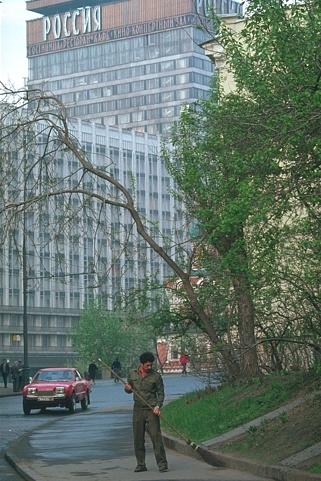
\includegraphics[width=0.9\linewidth]{figures/274007}
  \caption{Original image}
  \label{fig:sub1}
\end{subfigure}%
\begin{subfigure}{2.9cm}
  \centering
  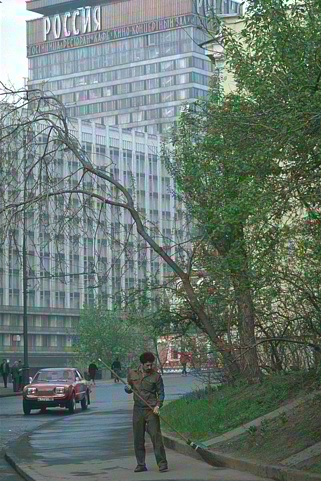
\includegraphics[width=0.9\linewidth]{figures/ac_shuffle_chrominance_76_274007}
  \caption{MOS $\simeq$ 5}
  \label{fig:sub2}
\end{subfigure}
\begin{subfigure}{2.9cm}
  \centering
  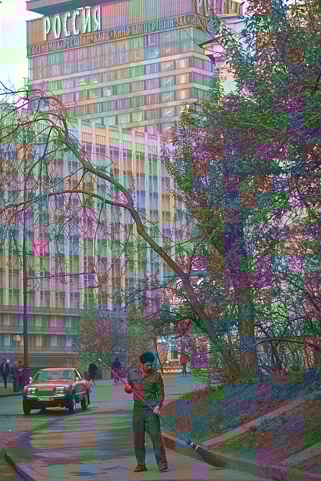
\includegraphics[width=0.9\linewidth]{figures/dc_shuffle_xor_chrominance_76_274007}
  \caption{MOS $\simeq$ 4}
  \label{fig:sub2}
\end{subfigure}
\begin{subfigure}{2.9cm}
  \centering
  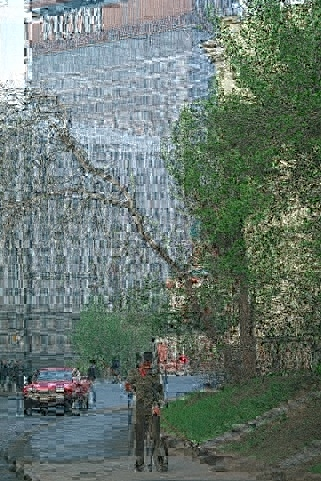
\includegraphics[width=0.9\linewidth]{figures/ac_xor_luminance_76_274007}
  \caption{MOS $\simeq$ 3}
  \label{fig:sub1}
\end{subfigure}%
\begin{subfigure}{2.9cm}
  \centering
  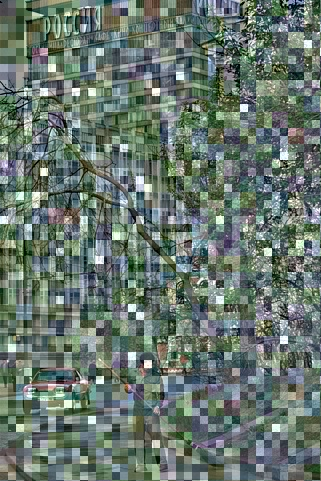
\includegraphics[width=0.9\linewidth]{figures/dc_shuffle_chrominance_luminance_76_274007}
  \caption{MOS $\simeq$ 2}
  \label{fig:sub2}
\end{subfigure}
\begin{subfigure}{2.9cm}
  \centering
  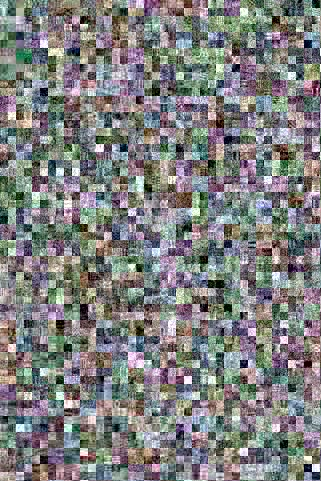
\includegraphics[width=0.9\linewidth]{figures/ac_dc_shuffle_xor_chrominance_luminance_76_274007}
  \caption{MOS $\simeq$ 1}
  \label{fig:sub2}
\end{subfigure}

\caption{Example of images for different selective encryption methods with their corresponding MOS}
\label{fig:images}
\end{figure*}

% \begin{figure}[ht]
% \centering
% \begin{subfigure}{4.3cm}
%   \centering
%   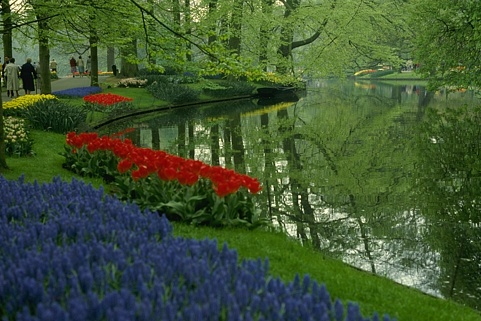
\includegraphics[width=0.9\linewidth]{figures/140055}
%   \caption{Original image}
%   \label{fig:sub1}
% \end{subfigure}%
% \begin{subfigure}{4.3cm}
%   \centering
%   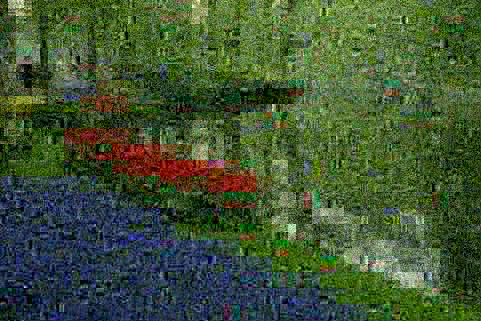
\includegraphics[width=0.9\linewidth]{figures/ac_shuffle_xor_chrominance_luminance_76_140055}
%   \caption{ac shuffle xor chroma luma}
%   \label{fig:sub2}
% \end{subfigure}
% \begin{subfigure}{4.3cm}
%   \centering
%   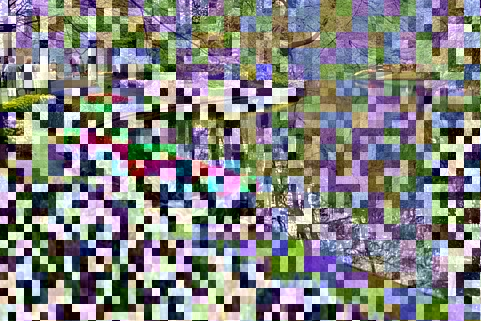
\includegraphics[width=0.9\linewidth]{figures/dc_xor_chrominance_luminance_76_140055}
%   \caption{dc xor chroma luma}
%   \label{fig:sub1}
% \end{subfigure}%
% \begin{subfigure}{4.3cm}
%   \centering
%   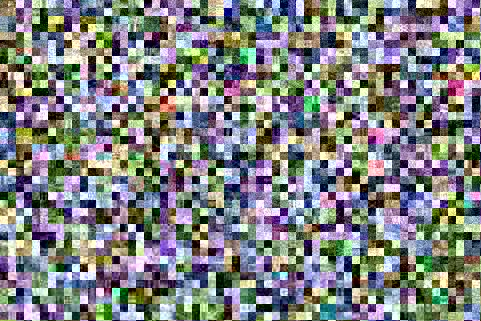
\includegraphics[width=0.9\linewidth]{figures/ac_dc_shuffle_xor_chrominance_luminance_76_140055}
%   \caption{All six parameters}
%   \label{fig:sub2}
% \end{subfigure}

% \caption{Example of different distortions}
% \label{fig:images}
% \end{figure}

The \textit{XOR} parameter corresponds to the method proposed by Puech \textit{et al.} \cite{fernandez2012advanced}. This method partially encrypts an image. This can be useful for partial visualisation, even if we only use it on the whole image, and it has two main strengths: it does not increase the size of the JPEG bitstream and it changes the DCT coefficients histogram. We encrypt the amplitude part of non null AC coefficients \textit{i.e.} the concatenation of the amplitude of each coefficient of each block $[A_0^i,..., A_k^i,..., A_0^n,..., A_k^n]$, where $n$ is the number of blocks. The amplitude sequence is denoted $A = [a_0,..., a_l]$ where $l$ is the number of amplitude bits. A standard stream cipher function is used to generate a pseudo-random sequence $E = [e_0,..., e_l]$ from a secret key. This sequence is XORed with the incoming plaintext to produce a ciphered sequence $\widetilde{A} = \widetilde{a}_0,..., \widetilde{a}_l$ where $\widetilde{a}_i = a_i \oplus e_i, i \in [0,l]$. The encrypted sequence is substitued to the amplitudes in the original bitstream.

The \textit{shuffle} parameter corresponds to a full inter-block shuffle (FIBS), proposed by Li and Yuan \cite{li2007leak}. This method can scramble DC coefficients as well as same frequency AC coefficients. As it scrambles all coefficients, run length encoding does not perform as well and the size of the image can increase. According to the authors, the use of all AC coefficients, zero as well as non-zero, creates a more secure image, less sensitive to jigsaw puzzle attacks \cite{}.

We used the training images from the BSDS500 \cite{amfm_pami2011} dataset as our input images for a total of $27 \times 200 = 5400$ cryptocompressed images.

% The 27 distortions are given in Appendix \ref{ann:distortions}, they are named according to the parameters enabled and are sorted by MOS, as explained in Section \ref{sec:evaluation}. They are later designated by their number for ease of use.

\section{Image evaluation}
\label{sec:evaluation}
We conducted our evaluation on \textit{N} different people. They had to give a score from 1 to 5 to the images, where 5 is the best score and 1 is the worst:\\\\
\textbf{1 :} The distortion is unbearable, nothing is visible\\
\textbf{2 :} \small{The distortion is very annoying, I can barely guess the content}\normalsize{}\\
\textbf{3 :} The distortion is annoying, but I can see the content\\
\textbf{4 :} The distortion is slightly annoying, but the content is clear\\
\textbf{5 :} The distortion is not annoying at all \\

An example of the 5 MOS is illustrated Fig.~\ref{fig:images}. They had to rate 81 images, three for each distortion. The sessions were 10 to 15 minutes long, depending on the person. Each image has been seen at most once by each user, to prevent them from recognising it and give it a higher score. The distortions order was shuffled differently for each evaluation and repeated three times in the same order. %We chose to have each distortion rated three times because during our preliminary tests, we saw that for the first few images, the user was not confident on the score to give to an image, confidence that improved as they saw more images and distortions. It allowed us to filter the outliers caused by the learning curve while still having a good amount of rating.

\begin{figure}[H]
  \centering
  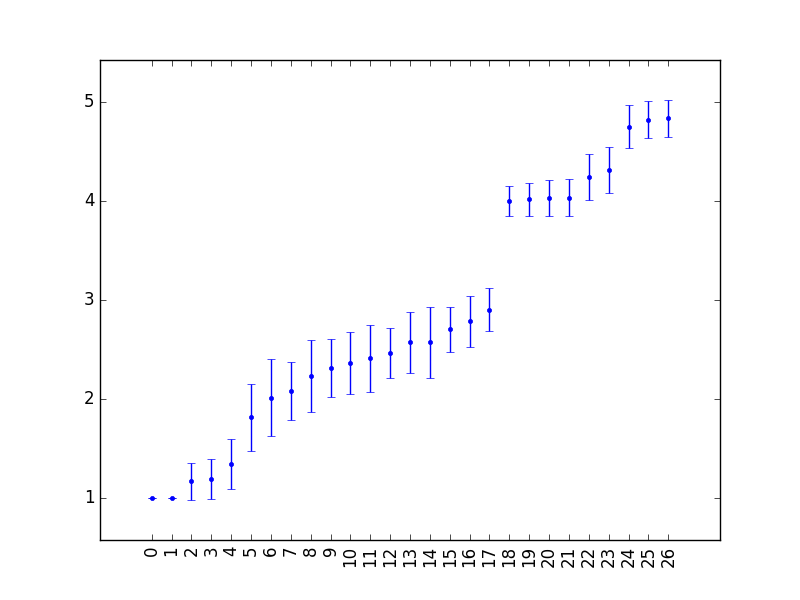
\includegraphics[width=8.5cm]{figures/mos}
  \vspace{-5mm}
  \caption{MOS for the 27 distortions.\label{fig:mos} }
\end{figure}

The images were evaluated in a dim room, on a \textit{details of the screen} screen, about $n$ meters away and around eyes level. The user could only see one image at a time, a new image shown once the previous had been rated.
The MOS obtained during the evaluation are given Fig. \ref{fig:mos}. % The name of the distortions are given in Appendix \ref{ann:distortions}.
We can see that after distortions $\#17$ there is a large gap in the MOS. This is due to the absence of the parameter $luminance$, the $shuffle$ and $XOR$ are only performed on the chrominance, hence the better ratings.
We give an overview of a few selected metrics we used for image analysis. For a more in-depth review, we refer the reader to \cite{hofbauer2016identifying}.

\textbf{PSNR:} Even though it is known that the PSNR is not well correlated with human judgment, it is still widely used due to its speed and ease of use. The range is [0; $+\infty$], where two identical images would have a PSNR of $+\infty$.

\textbf{SSIM\cite{wang2004image}:} (Structural Similarity Index Measure). A luminance score, a contrast score and a structure score are combined to obtain the actual SSIM score. It has a range of [0;1] where identical images have a score of 1.

\textbf{ESS\cite{mao2004security}:} (Edge Similarity Score). It uses non overlapping 8x8 block directions to compare images. With the range [0;1], a higher score reflects a less distorted image.

\textbf{LSS\cite{mao2004security}:} (Luminance Similarity Score). It uses non overlapping 8x8 block average luminance to compare images. With the range [-8.5; 1] for default parameters of $\alpha=0.1$ and $\beta=3$, a higher score reflects a less distorted image.

\textbf{NPCR\cite{chen2004symmetric, mao2004novel}:} It is the number of pixel changes between images. Its range is [0;100], where a fully encrypted image has a NPCR close to 100, where almost all the pixels changed.

\textbf{UACI\cite{chen2004symmetric, mao2004novel}:} It is the unified averaged changed intensity. It is the average intensity difference between two images. Its range is [0;100], where a fully encrypted image has a value close to 33.

% \textbf{Entropy :} It is the amount of information in an image, for an 8-bit image, so an entropy of 8 would be the target for a full encryption method. It ranges from 0 to 8 in this case.

% \textbf{Correlation :} The correlation coefficient ranges from 0 to 1, it is the average correlation of adjacent pixels in an image, where a natural image would be highly correlated and a fully encrypted image would have low correlation.


Our goal is to predict the rating a human would give to an image. In the best case scenario, a metric would be totally correlated with human rating and could be used to completely replace humans in image evaluation, this is however not the case, at least not for the metrics we selected, as shown in Fig.~\ref{fig:plots}.

\begin{figure}[ht]
\centering
\begin{subfigure}{4.3cm}
  \centering
  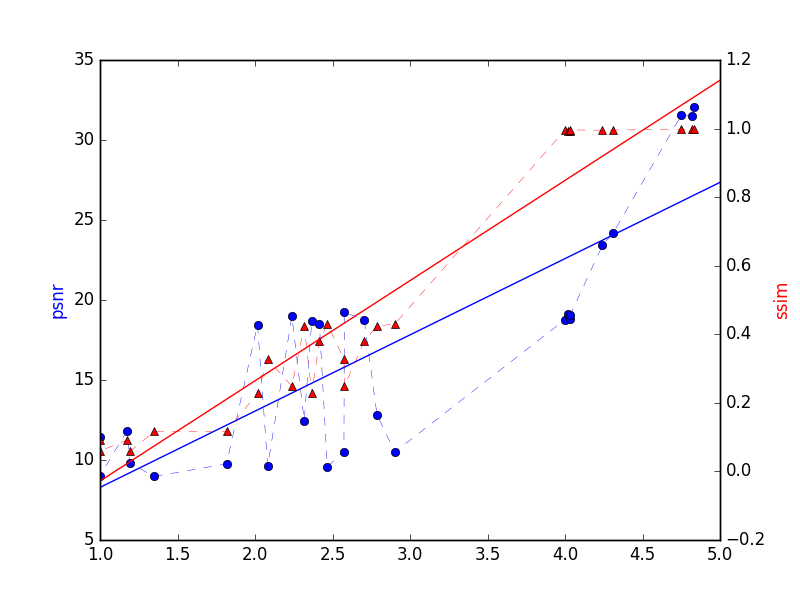
\includegraphics[width=1\linewidth]{figures/mos_ssim}
  \caption{\pbox{2.81cm}{Left axis : PSNR $\bigcirc$ Right axis : SSIM $\triangle$}}
  \label{fig:sub1}
\end{subfigure}%
\begin{subfigure}{4.3cm}
  \centering
  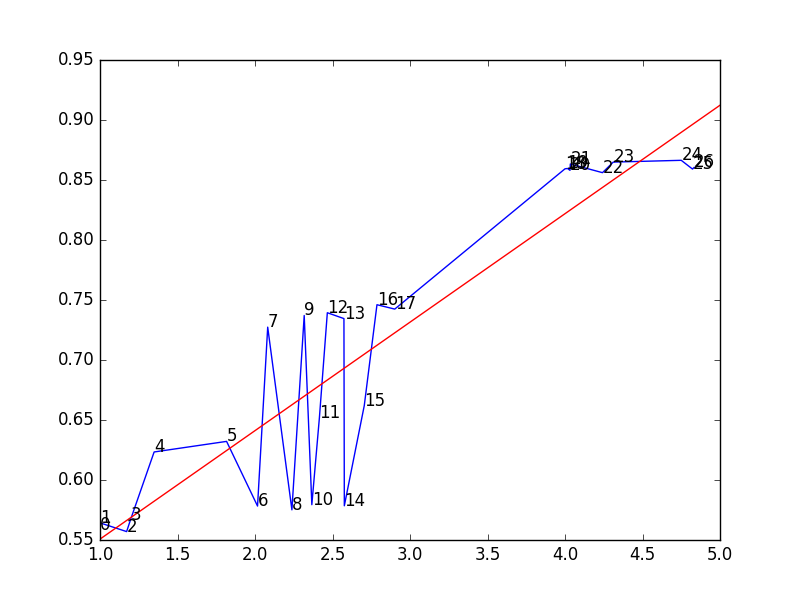
\includegraphics[width=1\linewidth]{figures/mos_ess}
  \caption{\pbox{2.81cm}{Left axis : LSS $\bigcirc$ Right axis : ESS $\triangle$}}
  \label{fig:sub2}
\end{subfigure}
\begin{subfigure}{4.3cm}
  \centering
  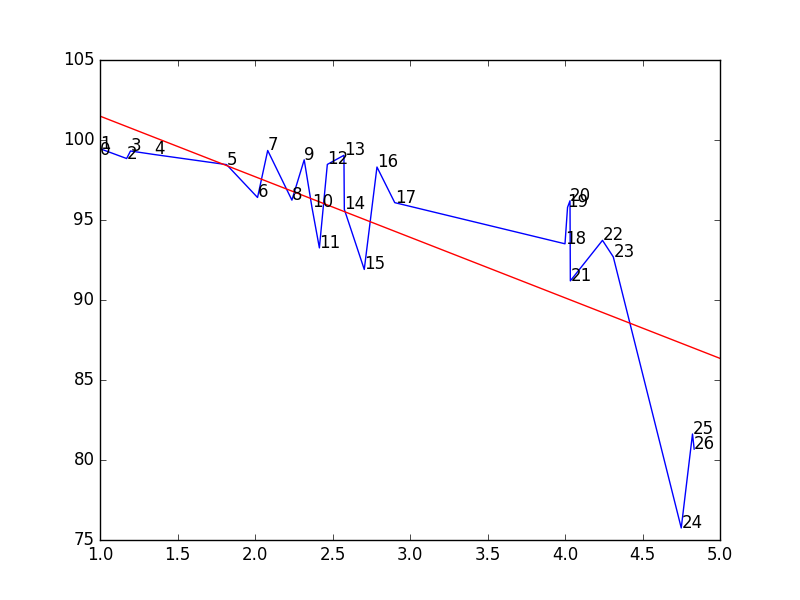
\includegraphics[width=1\linewidth]{figures/mos_npcr}
  \caption{\pbox{2.81cm}{Left axis : UACI $\bigcirc$ Right axis : NPCR $\triangle$}}
  \label{fig:sub3}
\end{subfigure}%
% \begin{subfigure}{4.3cm}
%   \centering
%   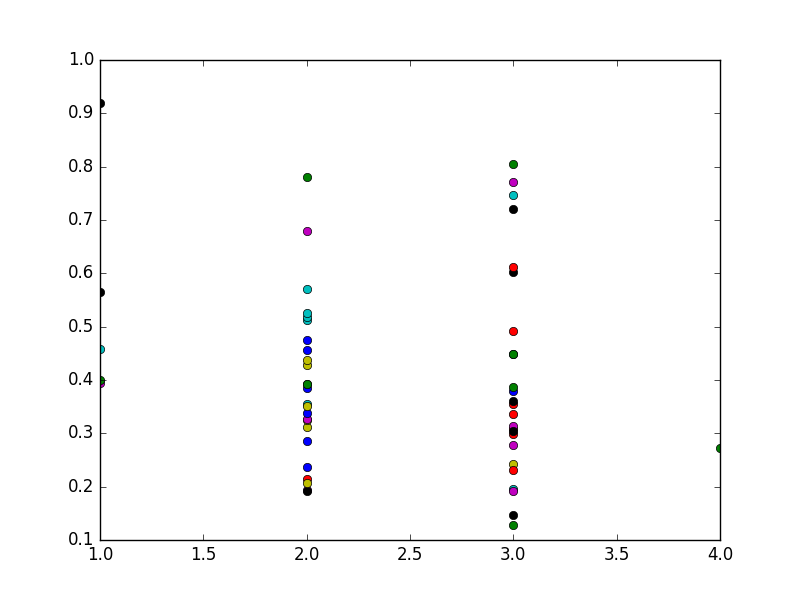
\includegraphics[width=1\linewidth]{figures/ssim_detail_11}
%   \caption{Breakdown of SSIM score for a single distortion}
%   % 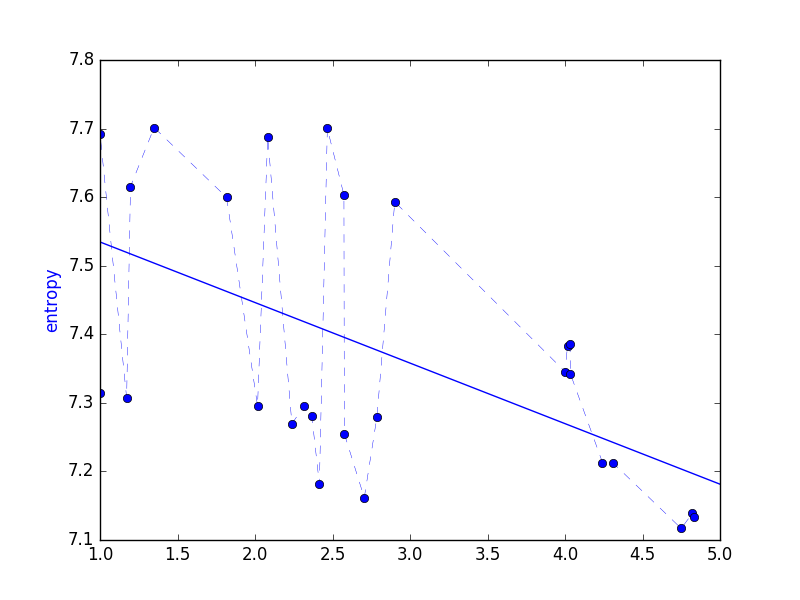
\includegraphics[width=1\linewidth]{figures/mos_entropy}
%   \label{fig:sub4}
% \end{subfigure}
\begin{subfigure}{4.3cm}
  \centering
  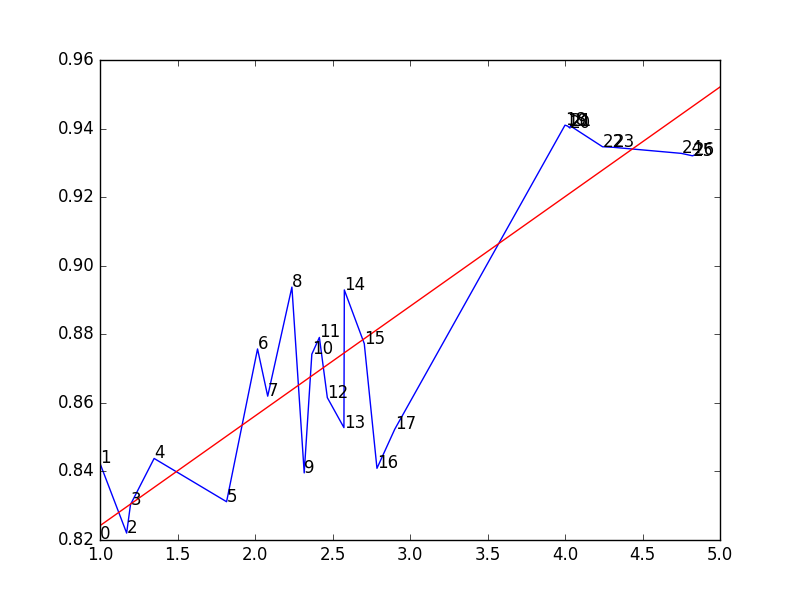
\includegraphics[width=1\linewidth]{figures/mos_corr_vert}
  \caption{\pbox{3.81cm}{Left axis : horizontal $\bigcirc$ Right axis : vertical $\triangle$ correlation}}
  \label{fig:sub5}
\end{subfigure}%

\caption{Plots of different metrics with the MOS on the x-axis, \ref{fig:sub1}: PSNR and SSIM, \ref{fig:sub2}: LSS and ESS, \ref{fig:sub3}: UACI and NPCR, \ref{fig:sub5}: horizontal and vertical correlation}
\label{fig:plots}
\end{figure}

% \begin{figure}[ht]
%   \centering
%   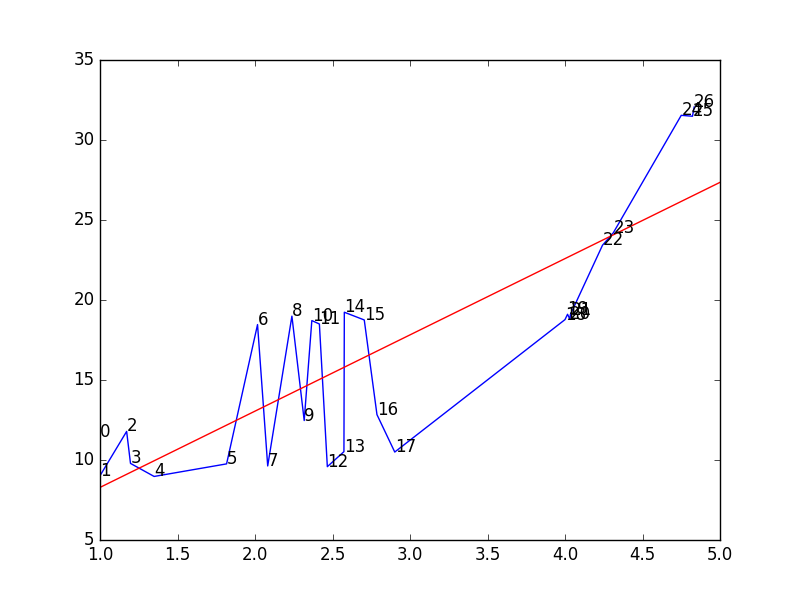
\includegraphics[width=8.5cm]{figures/mos_psnr}
%   \vspace{-5mm}
%   \caption{MOS on the x-axis and PSNR on the y-axis\label{fig:psnr} }
% \end{figure}

% \begin{figure}[ht]
%   \centering
%   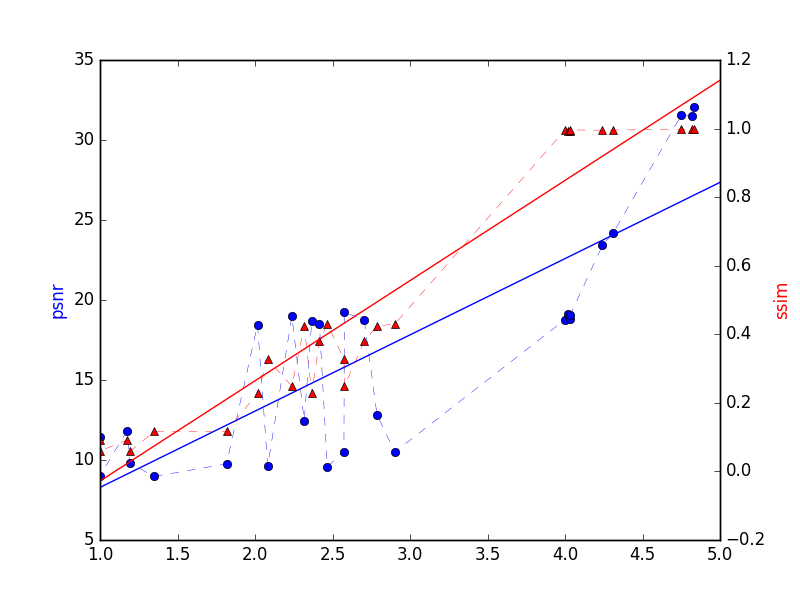
\includegraphics[width=8.5cm]{figures/mos_ssim}
%   \caption{MOS on the x-axis and SSIM on the y-axis\label{fig:ssim} }
%   \vspace{-5mm}
% \end{figure}
% \begin{figure}[ht]
%   \centering
%   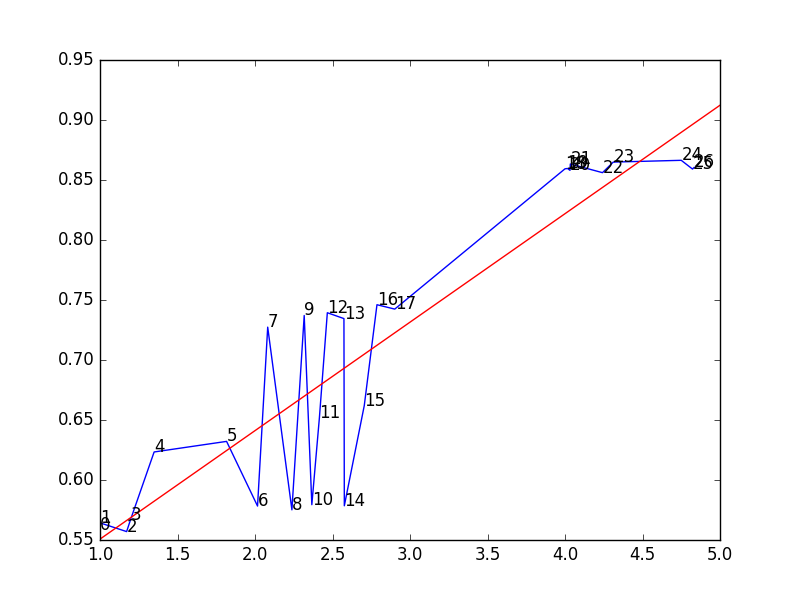
\includegraphics[width=8.5cm]{figures/mos_ess}
%   \caption{MOS on the x-axis and ESS on the y-axis\label{fig:ess} }
% \end{figure}
% \begin{figure}[ht]
%   \centering
%   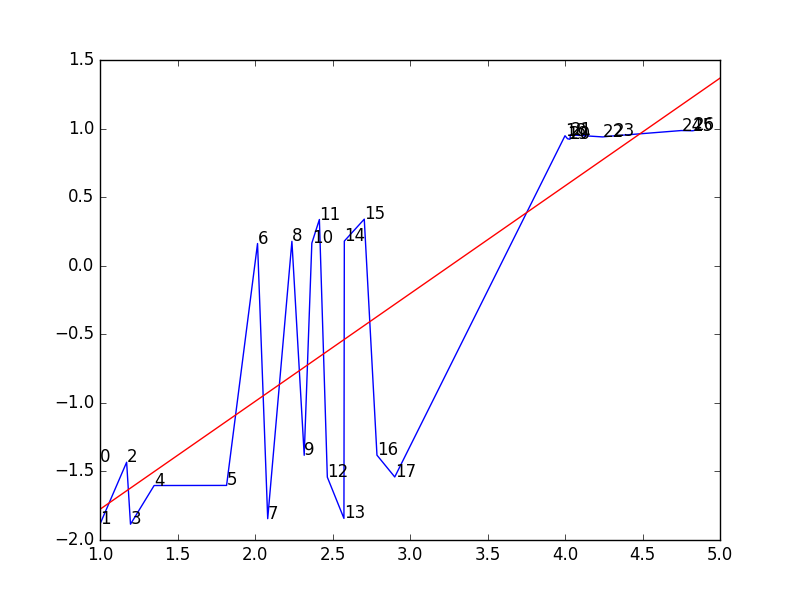
\includegraphics[width=8.5cm]{figures/mos_lss}
%   \caption{MOS on the x-axis and LSS on the y-axis\label{fig:lss} }
% \end{figure}
% \begin{figure}[ht]
%   \centering
%   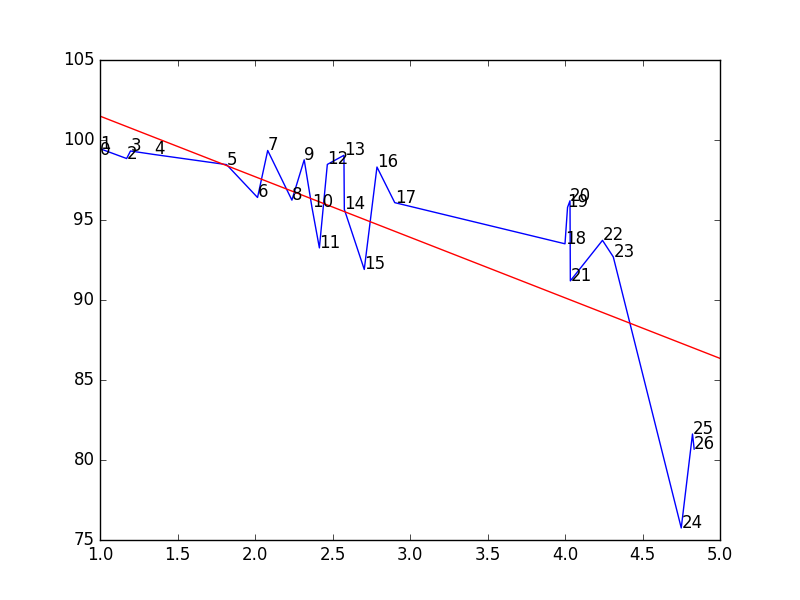
\includegraphics[width=8.5cm]{figures/mos_npcr}
%   \caption{MOS on the x-axis and NCPR on the y-axis\label{fig:npcr} }
% \end{figure}
% \begin{figure}[ht]
%   \centering
%   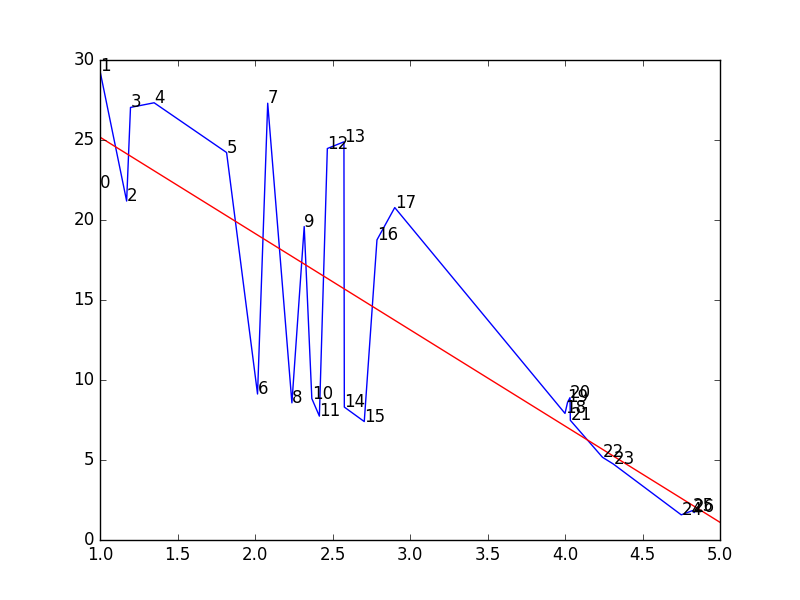
\includegraphics[width=8.5cm]{figures/mos_uaci}
%   \caption{MOS on the x-axis and UACI on the y-axis\label{fig:uaci} }
% \end{figure}
% \begin{figure}[ht]
%   \centering
%   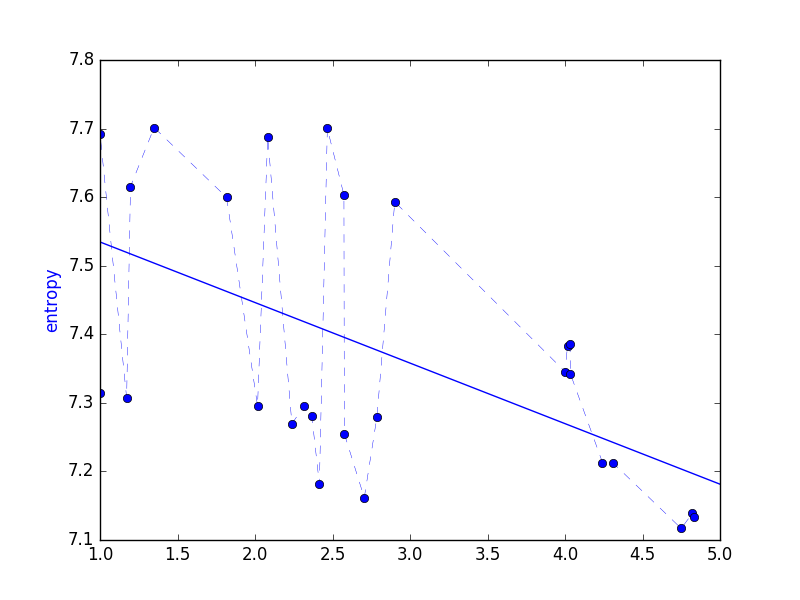
\includegraphics[width=8.5cm]{figures/mos_entropy}
%   \caption{MOS on the x-axis and entropy on the y-axis\label{fig:entropy} }
% \end{figure}
% \begin{figure}[ht]
%   \centering
%   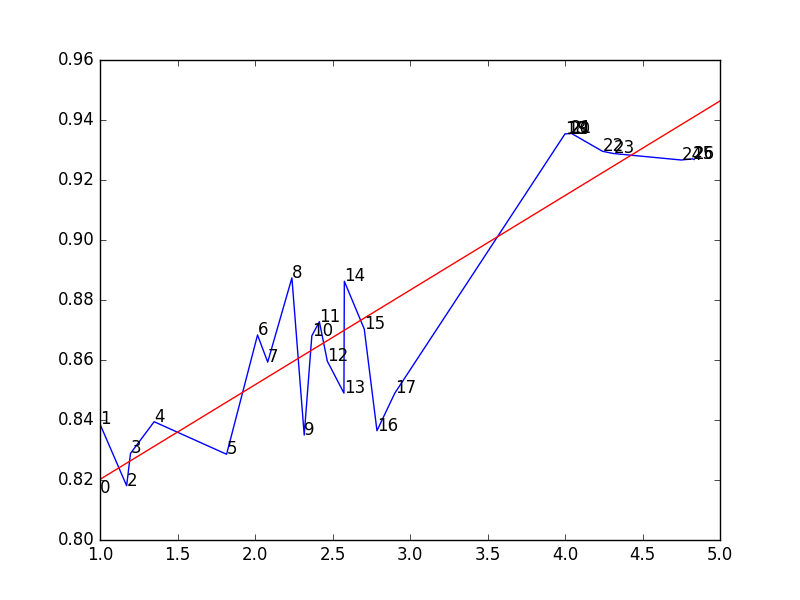
\includegraphics[width=8.5cm]{figures/mos_corr_horiz}
%   \caption{MOS on the x-axis and horizontal correlation on the y-axis\label{fig:correlation} }
% \end{figure}

As we can se from these figures, most metrics actually follow a rough line, but distortions $5$ to $17$ are problematic and prevent us from predicting the MOS. These distortions also happen to be between a MOS of 2 and 3, where the threshold for a confidential image would be. Even the SSIM, which is the most accurate metric in our experiment, fails to predict the MOS.%, as shown in Fig.~\ref{fig:sub4}. The SSIM ranges from 0 to 1, and from Fig.~\ref{fig:sub4}, we can see that for the same MOS the SSIM goes across almost all its range. A similar behavior is seen for the other metrics.

% \begin{figure}[ht]
%   \centering
%   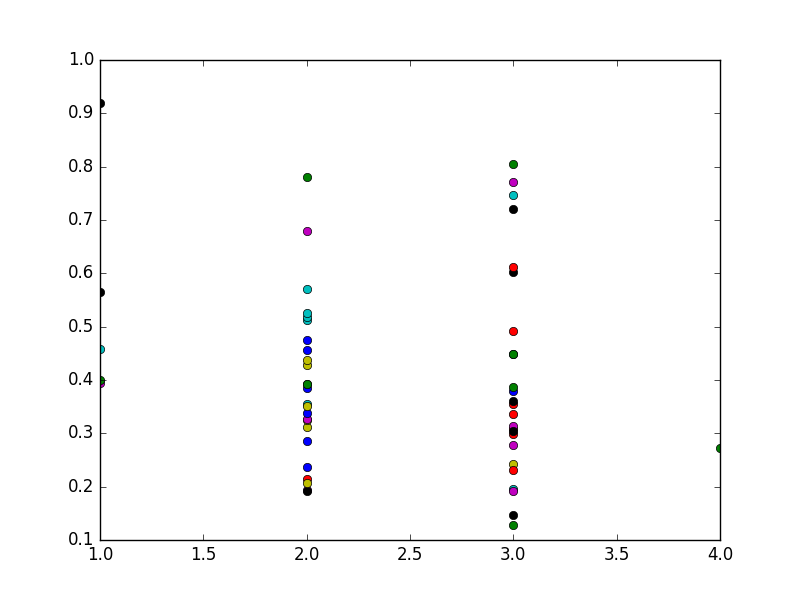
\includegraphics[width=8.5cm]{figures/ssim_detail_11}
%   \caption{Details of the MOS on the x-axis and the SSIM on the y-axis for the $11^{th}$ distortion \label{fig:ssim_detail_11} }
% \end{figure}

 %  \begin{table*}[ht]
%     \centering
%     \scalebox{0.8}{
%       \begin{tabular}{|c|c|c|c|c|c|c|c|c|c|c|}
%     \hline
%   index	&  MOS		&  psnr		&  entropy	&  corr\_horiz	&  corr\_vert	&  uaci		&  npcr		&  ssim		&  lss		&  ess		\\ \hline 
% 0	& 1.0 (0.0)	& 11.45 (2.72)	& 7.31 (0.39)	& 0.82 (0.05)	& 0.82 (0.05)	& 21.99 (6.42)	& 99.05 (0.73)	& 0.09 (0.07)	& -1.43 (0.52)	& 0.56 (0.2)	\\ \hline 
% 1	& 1.0 (0.0)	& 9.02 (1.93)	& 7.69 (0.16)	& 0.84 (0.04)	& 0.84 (0.04)	& 29.32 (6.34)	& 99.46 (0.18)	& 0.06 (0.04)	& -1.88 (0.57)	& 0.56 (0.19)	\\ \hline 
% 2	& 1.17 (0.38)	& 11.79 (2.82)	& 7.31 (0.39)	& 0.82 (0.05)	& 0.82 (0.05)	& 21.19 (6.46)	& 98.84 (1.19)	& 0.09 (0.07)	& -1.43 (0.52)	& 0.56 (0.2)	\\ \hline 
% 3	& 1.2 (0.4)	& 9.79 (2.38)	& 7.62 (0.23)	& 0.83 (0.04)	& 0.83 (0.05)	& 27.03 (6.75)	& 99.31 (0.38)	& 0.06 (0.04)	& -1.88 (0.57)	& 0.57 (0.19)	\\ \hline 
% 4	& 1.35 (0.51)	& 8.97 (1.97)	& 7.7 (0.19)	& 0.84 (0.04)	& 0.84 (0.04)	& 27.33 (6.32)	& 99.09 (0.31)	& 0.12 (0.09)	& -1.6 (0.57)	& 0.62 (0.2)	\\ \hline 
% 5	& 1.82 (0.67)	& 9.76 (2.42)	& 7.6 (0.27)	& 0.83 (0.05)	& 0.83 (0.04)	& 24.22 (6.68)	& 98.46 (0.95)	& 0.12 (0.09)	& -1.6 (0.57)	& 0.63 (0.19)	\\ \hline 
% 6	& 2.02 (0.78)	& 18.46 (3.04)	& 7.3 (0.41)	& 0.87 (0.07)	& 0.88 (0.07)	& 9.12 (3.17)	& 96.41 (3.52)	& 0.23 (0.12)	& 0.16 (0.2)	& 0.58 (0.18)	\\ \hline 
% 7	& 2.08 (0.58)	& 9.63 (2.14)	& 7.69 (0.18)	& 0.86 (0.03)	& 0.86 (0.03)	& 27.3 (6.51)	& 99.35 (0.23)	& 0.33 (0.13)	& -1.84 (0.55)	& 0.73 (0.16)	\\ \hline 
% 8	& 2.24 (0.73)	& 18.99 (3.09)	& 7.27 (0.42)	& 0.89 (0.06)	& 0.89 (0.06)	& 8.57 (3.02)	& 96.24 (3.59)	& 0.25 (0.13)	& 0.18 (0.2)	& 0.58 (0.19)	\\ \hline 
% 9	& 2.32 (0.59)	& 12.47 (3.03)	& 7.3 (0.4)	& 0.83 (0.04)	& 0.84 (0.04)	& 19.59 (6.28)	& 98.76 (0.9)	& 0.42 (0.14)	& -1.38 (0.51)	& 0.74 (0.16)	\\ \hline 
% 10	& 2.37 (0.63)	& 18.71 (3.13)	& 7.28 (0.42)	& 0.87 (0.07)	& 0.87 (0.07)	& 8.84 (3.19)	& 95.83 (4.29)	& 0.23 (0.12)	& 0.16 (0.2)	& 0.58 (0.18)	\\ \hline 
% 11	& 2.42 (0.68)	& 18.5 (3.03)	& 7.18 (0.48)	& 0.87 (0.07)	& 0.88 (0.07)	& 7.74 (2.99)	& 93.26 (5.3)	& 0.38 (0.16)	& 0.34 (0.22)	& 0.65 (0.18)	\\ \hline 
% 12	& 2.47 (0.5)	& 9.58 (2.17)	& 7.7 (0.2)	& 0.86 (0.03)	& 0.86 (0.03)	& 24.47 (6.36)	& 98.47 (0.5)	& 0.43 (0.14)	& -1.54 (0.57)	& 0.74 (0.15)	\\ \hline 
% 13	& 2.57 (0.61)	& 10.52 (2.67)	& 7.6 (0.25)	& 0.85 (0.03)	& 0.85 (0.03)	& 24.89 (6.89)	& 99.04 (0.5)	& 0.33 (0.13)	& -1.84 (0.55)	& 0.73 (0.15)	\\ \hline 
% 14	& 2.58 (0.72)	& 19.24 (3.17)	& 7.26 (0.43)	& 0.89 (0.06)	& 0.89 (0.06)	& 8.31 (3.03)	& 95.67 (4.37)	& 0.25 (0.13)	& 0.18 (0.2)	& 0.58 (0.18)	\\ \hline 
% 15	& 2.7 (0.46)	& 18.75 (3.11)	& 7.16 (0.49)	& 0.87 (0.07)	& 0.88 (0.07)	& 7.4 (2.99)	& 91.91 (6.31)	& 0.38 (0.16)	& 0.34 (0.22)	& 0.66 (0.18)	\\ \hline 
% 16	& 2.79 (0.52)	& 12.84 (3.13)	& 7.28 (0.41)	& 0.84 (0.04)	& 0.84 (0.04)	& 18.76 (6.29)	& 98.31 (1.48)	& 0.42 (0.14)	& -1.38 (0.51)	& 0.75 (0.15)	\\ \hline 
% 17	& 2.9 (0.43)	& 10.5 (2.71)	& 7.59 (0.29)	& 0.85 (0.03)	& 0.85 (0.03)	& 20.78 (6.65)	& 96.08 (1.75)	& 0.43 (0.14)	& -1.54 (0.57)	& 0.74 (0.15)	\\ \hline 
% 18	& 4.0 (0.31)	& 18.77 (3.9)	& 7.35 (0.37)	& 0.94 (0.04)	& 0.94 (0.04)	& 7.91 (3.4)	& 93.51 (3.95)	& 1.0 (0.01)	& 0.95 (0.08)	& 0.86 (0.1)	\\ \hline 
% 19	& 4.02 (0.34)	& 19.11 (4.1)	& 7.38 (0.35)	& 0.94 (0.04)	& 0.94 (0.04)	& 8.6 (3.72)	& 95.79 (3.12)	& 0.99 (0.01)	& 0.93 (0.1)	& 0.86 (0.1)	\\ \hline 
% 20	& 4.03 (0.36)	& 18.79 (3.93)	& 7.39 (0.34)	& 0.94 (0.04)	& 0.94 (0.04)	& 8.9 (3.74)	& 96.2 (2.89)	& 0.99 (0.01)	& 0.92 (0.1)	& 0.86 (0.1)	\\ \hline 
% 21	& 4.03 (0.37)	& 19.08 (4.08)	& 7.34 (0.38)	& 0.94 (0.04)	& 0.94 (0.04)	& 7.48 (3.33)	& 91.2 (4.87)	& 1.0 (0.01)	& 0.95 (0.07)	& 0.86 (0.1)	\\ \hline 
% 22	& 4.24 (0.46)	& 23.42 (4.04)	& 7.21 (0.44)	& 0.93 (0.05)	& 0.93 (0.05)	& 5.17 (2.26)	& 93.73 (3.84)	& 1.0 (0.01)	& 0.94 (0.08)	& 0.86 (0.1)	\\ \hline 
% 23	& 4.31 (0.46)	& 24.2 (4.26)	& 7.21 (0.45)	& 0.93 (0.05)	& 0.93 (0.05)	& 4.75 (2.18)	& 92.69 (4.34)	& 1.0 (0.01)	& 0.95 (0.07)	& 0.86 (0.09)	\\ \hline 
% 24	& 4.75 (0.43)	& 31.54 (3.66)	& 7.12 (0.5)	& 0.93 (0.05)	& 0.93 (0.05)	& 1.57 (0.7)	& 75.75 (10.71)	& 1.0 (0.0)	& 0.99 (0.03)	& 0.87 (0.09)	\\ \hline 
% 25	& 4.82 (0.38)	& 31.48 (3.71)	& 7.14 (0.48)	& 0.93 (0.05)	& 0.93 (0.05)	& 1.84 (0.83)	& 81.63 (9.59)	& 1.0 (0.0)	& 0.98 (0.04)	& 0.86 (0.1)	\\ \hline 
% 26	& 4.83 (0.37)	& 32.06 (3.75)	& 7.13 (0.49)	& 0.93 (0.05)	& 0.93 (0.05)	& 1.72 (0.79)	& 80.68 (10.02)	& 1.0 (0.0)	& 0.99 (0.03)	& 0.86 (0.1)	\\ \hline 
%       \end{tabular}
%     }
%         \caption{Results for the 27 distortions \label{fig:table}}
%     \end{table*}
% \section{REFERENCES}
% \label{sec:ref}

% \appendix
% \section{Distortions}
% \label{ann:distortions}
% \begin{enumerate}
%   \itemsep-0.5em 
%   \setcounter{enumi}{-1}
% \item ac\_dc\_shuffle\_chrominance\_luminance
% \item ac\_dc\_shuffle\_xor\_chrominance\_luminance
% \item ac\_dc\_shuffle\_luminance
% \item ac\_dc\_shuffle\_xor\_luminance
% \item ac\_dc\_xor\_chrominance\_luminance
% \item ac\_dc\_xor\_luminance
% \item ac\_shuffle\_xor\_chrominance\_luminance
% \item dc\_shuffle\_xor\_chrominance\_luminance
% \item ac\_shuffle\_chrominance\_luminance
% \item dc\_shuffle\_chrominance\_luminance
% \item ac\_shuffle\_xor\_luminance
% \item ac\_xor\_chrominance\_luminance
% \item dc\_xor\_chrominance\_luminance
% \item dc\_shuffle\_xor\_luminance
% \item ac\_shuffle\_luminance
% \item ac\_xor\_luminance
% \item dc\_shuffle\_luminance
% \item dc\_xor\_luminance
% \item ac\_dc\_xor\_chrominance
% \item dc\_shuffle\_xor\_chrominance
% \item ac\_dc\_shuffle\_xor\_chrominance
% \item dc\_xor\_chrominance
% \item ac\_dc\_shuffle\_chrominance
% \item dc\_shuffle\_chrominance
% \item ac\_xor\_chrominance
% \item ac\_shuffle\_xor\_chrominance
% \item ac\_shuffle\_chrominance
% \end{enumerate}

% List and number all bibliographical references at the end of the
% paper. The references can be numbered in alphabetic order or in
% order of appearance in the document. When referring to them in
% the text, type the corresponding reference number in square
% brackets as shown at the end of this sentence \cite{C2}. An
% additional final page (the fifth page, in most cases) is
% allowed, but must contain only references to the prior
% literature.

% References should be produced using the bibtex program from suitable
% BiBTeX files (here: strings, refs, manuals). The IEEEbib.bst bibliography
% style file from IEEE produces unsorted bibliography list.
% -------------------------------------------------------------------------
\section{Visual saliency as a means to evaluate image}
\label{sec:metric}
In this section, we present the new metric we designed, the results we obtained and their analysis. Our metric is based on the visual saliency in images, and more specifically, and saliency map, a grayscale image where less salient pixels are darker than more salient pixels in the original image. The visual saliency is interesting in our case for image quality assessment because we want to know whether the meaning of the content of an image is accessible. According to \cite{itti1998model}, important information is located in salient areas. Our reasoning is twofold: if salient areas are consistent in both the original and the processed image, the same amount of information is present in the images and the content is readily available, and if no salient areas can be found, as important information is located in salient areas, then the content is hidden. We try to compute to which extent the visual saliency of two images are similar to extract a score.

\paragraph*{}
Let $M_o$  be the saliency map of the original image and $M_p$ be the saliency map of the processed image. A threshold is applied to $M_o$ and $M_p$ to only keep the most salient areas of each image, the best threshold has been experimentally found (Fig~\ref{}) to be $5\%$ more salient areas. Two binary images are thus created, $B_o$ from $M_o$ and $B_p$ from $M_p$. A first value is computed as such:
$$
v = \frac{\sum_{i=0}^{width}\sum_{j=0}^{height}{f(B_o(i,j), B_p(i,j))}}{sum(B_o)},
$$

where $f(.,.)$ is:

$$
f(x,y) = \begin{cases}
    1, & \textbf{if}\ x = 1\ \textbf{and}\ y = 1\\ 
    0 & Otherwise,
  \end{cases}
$$

and $sum(B_o)$ is actually the number of pixels of value 1.

\paragraph*{}
\begin{figure}[H]
  \centering
\end{figure}

\begin{figure}[ht]
\centering
\begin{subfigure}{4.0cm}
  \centering
  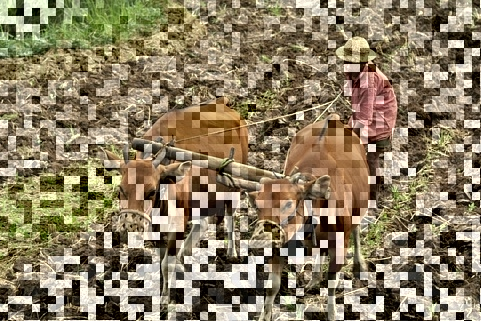
\includegraphics[width=0.95\linewidth]{figures/dc_xor_luminance_76_202012}
  \caption{\pbox{2.6cm}{\footnotesize{$XOR$ on the luma DC coefficients\label{fig:noise} }}}
  \label{fig:dc_xor}
\end{subfigure}%
\begin{subfigure}{4.0cm}
  \centering
  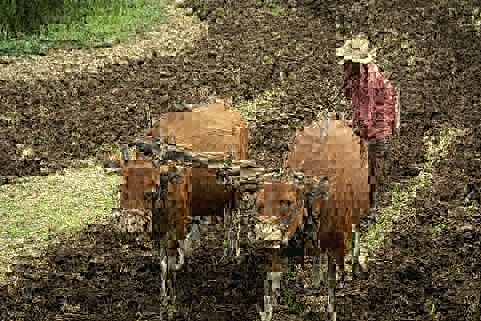
\includegraphics[width=0.95\linewidth]{figures/ac_xor_luminance_76_202012}
  \caption{\pbox{2.6cm}{\footnotesize{$XOR$ on the luma AC coefficients\label{fig:noise} }}}
  \label{fig:ac_xor}
\end{subfigure}
\caption{Global noise caused by a $XOR$ on DCT coefficients\label{fig:vs_bad}}
\end{figure}


% The main problem with the visual saliency is that it does not perform well on images with a global noise, such as a $XOR$ on the DC coefficients of the luminance channel for example (Fig~\ref{fig:noise}). In an attempt to address this problem, we introduce a second value, computed using the sobel edge detector \cite{}.

\paragraph*{}
% This technique, however intersting on paper, works well for both ends of the MOS spectrum but is not able to predict the MOS for mid-quality images, around a MOS of 2 or 3.
This technique works well for high or low quality images, where our metric accurately predicts the MOS. The results are however not as good for mid quality images, when the MOS is around 2-3. Because of this, we can only tell that an image is either fully confidential or not very to not confidential at all, but not to which degree it is confidential.

This is due to the fact that we are not able to compute a meaningful saliency map on images with a global, patterned noise, such as such as a $XOR$ on the DC coefficients of the luminance channel for example (Fig~\ref{fig:dc_xor}). Another problem we encountered is that the the visual saliency performs too well on distorted images where the global structure is intact but ..., typically when a $XOR$ is applied to the AC coefficients of the luminance channel (Fig~\ref{fig:ac_xor}).

Because of these two types of distortions, and their variations, using only the visual saliency is not a realistic approach for automatic image evaluation. We introduce a second score, based on the Sobel operator in an attempt to stabilize our first score.



\section{Conclusion}
\label{sec:conclusion}

\newpage
\bibliographystyle{IEEEbib}
\bibliography{strings,refs}

\end{document}
